\title{Warm-Up for March 9th, 2022}
\author{Dr. Jordan Hanson - Whittier College Dept. of Physics and Astronomy}
\date{\today}
\documentclass[12pt]{article}
\usepackage[a4paper, total={18cm, 27cm}]{geometry}
\usepackage{graphicx}
\usepackage{amsmath}
\usepackage{bm}
\begin{document}
\maketitle

\section{Memory Bank}

\begin{enumerate}
\item Hyperbolic cosine: $2\cosh(kx) = \exp(k x) + \exp(-kx)$.
\item Single general solution to the Laplacian in Cartesian coordinates:
\begin{equation}
V(x,y) = \left( A\exp(kx) + B\exp(-kx) \right) \left( C\sin(ky) + D\cos(ky) \right) \label{eq:sol}
\end{equation}
\end{enumerate}

\section{Solutions to the Laplacian for Potential}

\textit{Supposed two infinitely long grounded metal plates are situated in the $xz$ plane at $y=0$ and $y=a$, and have widths $2b$.  Suppose also that two infinitely long plates of width $a$ are situated in the $xy$ plane at $x = \pm b$, each with voltage $V_0$.  See Fig. \ref{fig:pipe}.}

\begin{itemize}
\item In your own words, why does the single solution of the Laplacian reduce to Eq. \ref{eq:sol}?  Determine the four boundary conditions of $V(x,y)$. \\
\item In your own words, why must $A = B$ given these boundary conditions? \\
\item Show that the general sum of solutions is
\begin{equation}
V(x,y) = \sum_i^{\infty} C_n \cosh(n\pi x/a) \sin(n\pi y/a) \label{eq:sol2}
\end{equation} \\
\item Use Fourier's Trick with $x = b$ to determine the $C_n$ coefficients.
\end{itemize}

\begin{figure}
\centering
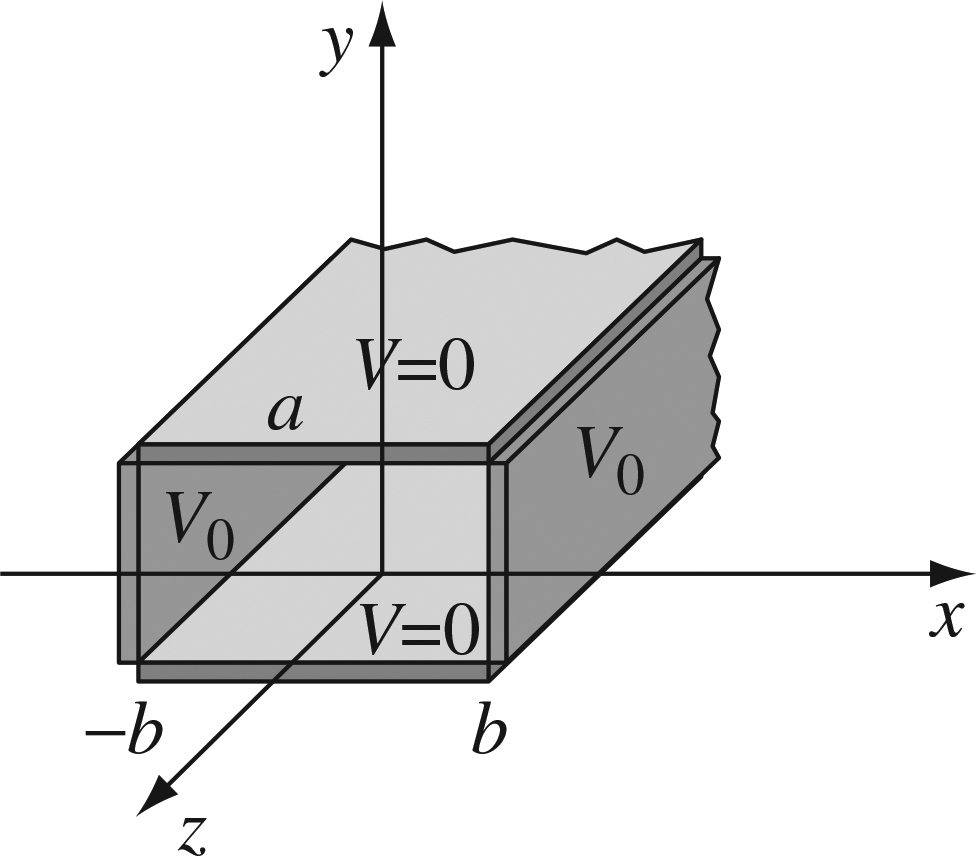
\includegraphics[width=0.25\textwidth]{figures/3_20.jpg} \hspace{1cm}
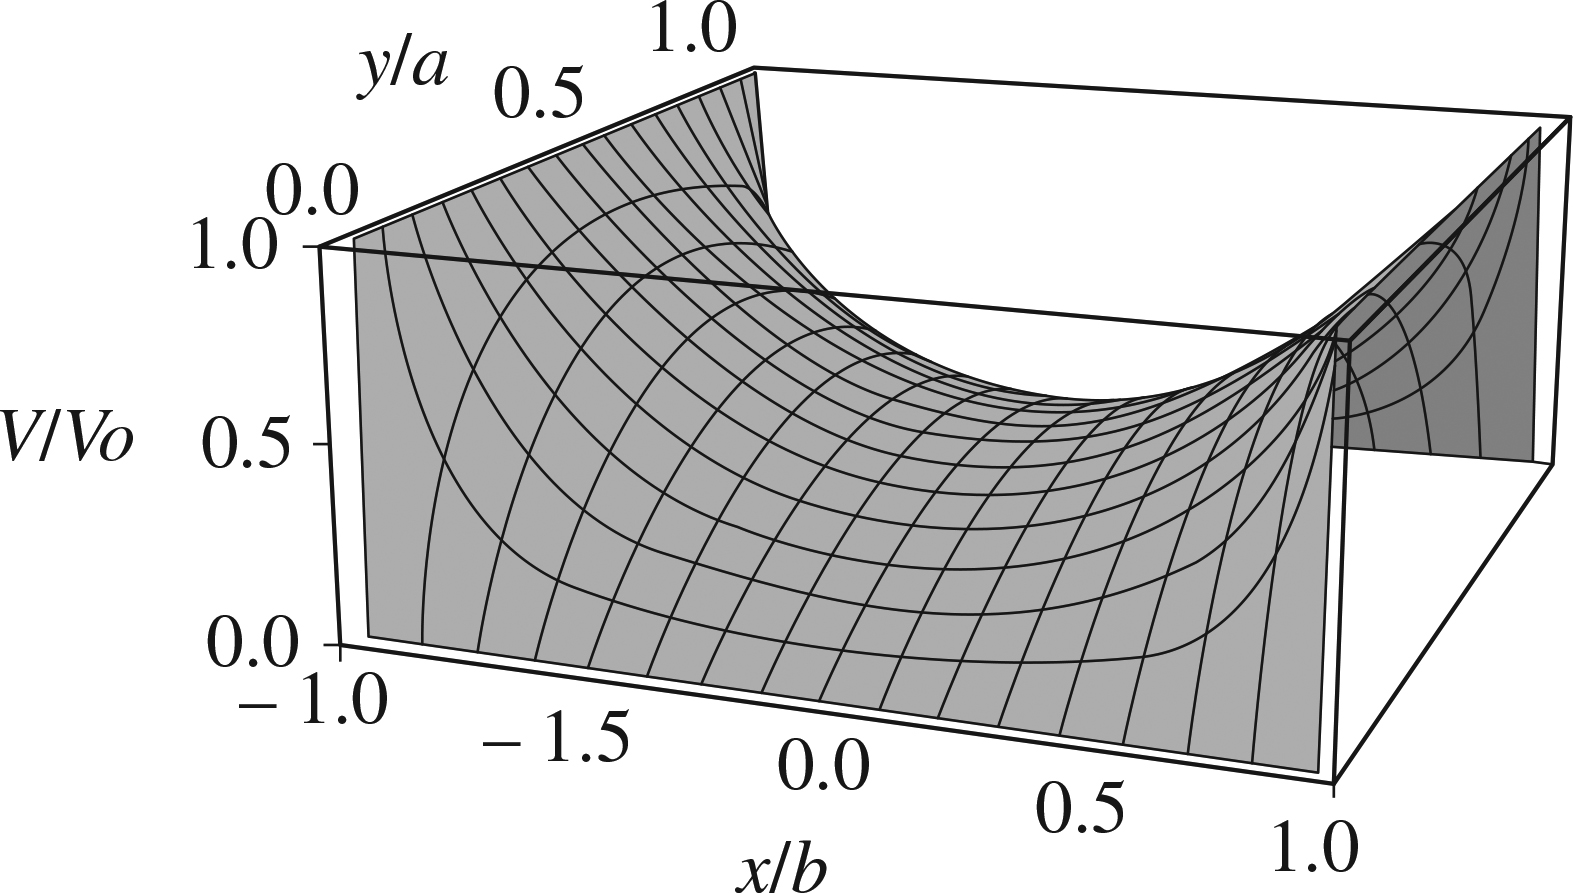
\includegraphics[width=0.25\textwidth]{figures/3_21.jpg}
\caption{\label{fig:pipe} (Left) A rectangular pipe with two sides grounded and two sides at constant potential $V_0$. (Right) The shape of the solution (Eq. \ref{eq:sol2}).}
\end{figure}

\end{document}